\chapter{Trabalhos Correlatos} % TODO: Comentar mais sobre estudos que apresentam o impacto de diferentes técnicas de fine-tuning

Nesta seção serão apresentados os trabalhos similares a este para realizar comparações e apresentar melhor o estado da arte nessa linha de pesquisa.

\section{Classificação Automática de Lesões de Pele}

A utilização de \ac{IA} na detecção e classificação de lesões de pele tem se tornado cada vez mais relevante ao longo das últimas décadas. Historicamente, os maiores
avanços nessa área começaram com advento da aprendizagem profunda e das \acp{CNN} \cite{li2019artificial}. A maioria das técnicas tenta classificar o câncer de pele, mais
especificamente o melanoma, \ac{CBC} e \ac{CEC}. Porém, as técnicas desenvolvidas no contexto da classificação do câncer de pele também são úteis na classificação de
outras doenças \cite{okuboyejo2018review}.

O trabalho de \textcite{skin_cancer_ai} apresenta que os conjuntos de dados mais comuns na área são o HAM10000 e os fornecidos pela \ac{ISIC}. Além disso, \acp{CNN} ainda
dominam a área como a principal forma de implementar um sistema de classificação de lesões, atingindo entre 80\% e 99\% de acurácia. Cerca de 48,12\% dos conjuntos de
dados utilizam imagens de dermatoscopia, enquanto 33,33\% deles usam imagens macroscópicas, como as de aproximação e panorâmicas mencionadas na
\autoref{sec:skin_lesion_images}. Os outros 18,52\% se tratam de conjuntos com diversas modalidades de imagens, como imagens de ultrasonografia, multiespectrais e outras.

\section{Classificação com ViTs}

Vários modelos de classificação de lesões baseados em \acp{ViT} foram propostos desde a introdução dessa arquitetura. A pesquisa de \textcite{khan2023identifying}
apresenta o cenário da utilização de \acp{ViT} nessa área. Muitas implementações seguem um modelo híbrido de \ac{ViT} e \ac{CNN}, combinando as capacidades das duas
arquiteturas.

Uma desvantagem das \acp{CNN} é a falta de entendimento de relações espaciais de longa distância em imagens de lesões de pele. Entretanto, \acp{ViT} conseguem resolver
esse problema, capturando as relações espaciais através do mecanismo de atenção. Mas, devido ao processo de divisão da imagem em seções de baixa resolução, \acp{ViT}
acabam tendo um desempenho pior, pois há uma perda de informações sobre detalhes mais finos. Nesse contexto, a utilização de modelos híbridos resolve esses problemas.
Uma dessas arquiteturas híbridas é a \textit{TransUNet}, combinando transformadores e \textit{U-Nets}, que conforme evidenciado por \textcite{gulzar2022skin}, consegue
atingir uma acurácia de 92,11\% na classificação de lesões de pele através do treinamento com o conjunto de dados \ac{ISIC}-2018.

\section{Classificação com MLLMs}

\acp{MLLM} vêm sendo aplicados no contexto da dermatologia nos últimos anos. O \ac{GPT}-4V e o \ac{LLaVA} são dois modelos proeminentes na resolução de tarefas
visuais. Em um estudo de \textcite{cirone2024assessing}, é analisada a eficácia do uso desses modelos na identificação de melanomas em diferentes tons de pele.

Os testes foram feitos com os conjuntos de dados MClass-D, Dermnet NZ e imagens de livros de dermatologia, contendo imagens macroscópicas com resolução de
\begin{math}900 \times 1600\end{math} pixels. Para cada imagem, foram feitas 20 perguntas em relação às suas características, sendo que cada modelo foi testado com 3
imagens, resultando num total de 60 pares de pergunta e imagem por modelo. As imagens também tiveram suas cores modificadas para avaliar o impacto da coloração na
identificação de melanomas.

% TODO: Comentar sobre o modelo do Marques (http://sibgrapi.sid.inpe.br/col/sid.inpe.br/sibgrapi/2024/08.28.22.28/doc/Marques-125.pdf) e o SkinDiseaseChat

No fim, o \ac{GPT}-4V atingiu uma acurácia de 85\% e o \ac{LLaVA} atingiu apenas 45\%. O modelo \ac{LLaVA} não conseguiu identificar melanomas corretamente quando as
imagens tinham suas cores modificadas e também não conseguiu identificar detalhes como ulcerações ou sangramentos. Um detalhe importante é que ambos os modelos são
generalistas e não são treinados com um foco na classificação de lesões de pele.

O \textit{benchmark} OmniMedVQA de \textcite{hu2024omnimedvqa} traz dados sobre o desempenho de \acp{MLLM} em diferentes tarefas visuais da medicina. Em particular, os
testes apresentam as pontuações de diversos modelos na área de dermatologia, como pode ser visto na \autoref{tab:omnimedvqa_dermatology_results}.

\begin{table}[ht]
    \caption{\small Pontuação no \textit{benchmark} OmniMedVQA em dermatologia. A primeira seção de linhas contém modelos generalistas e a outra contém modelos
        especializados na área médica.}
    \centering
    \begin{tabular}{l|c}
        \hline
        Modelo                  & Pontuação em dermatologia \\ \hline
        InstructBLIP            & 61,86                     \\
        \ac{LLaMA}\_Adapter\_v2 & 51,43                     \\
        \ac{LLaVA}              & 49,67                     \\
        PGTrans                 & 44,66                     \\
        Otter                   & 42,66                     \\
        BLIP-2                  & 41,07                     \\
        Mini\ac{GPT}-4          & 40,09                     \\
        mPLUG-Owl               & 35,98                     \\ \hline
        \ac{LLaVA}-Med          & 44,90                     \\
        RadFM                   & 39,03                     \\
        Med-Flamingo            & 32,33                     \\
        MedVInT                 & 29,13                     \\ \hline
    \end{tabular}
    \label{tab:omnimedvqa_dermatology_results}
    \fonte{\textcite{hu2024omnimedvqa}}
\end{table}

Nas subseções abaixo, serão apresentados alguns modelos que focam em problemas relacionados à classificação de lesões de pele.

\subsection{SkinGPT-4}

Esse modelo foi proposto e desenvolvido por \textcite{zhou2023skingpt} e se baseia no Mini\ac{GPT}-4, um \ac{MLLM} composto por um \ac{ViT} com um \textit{Q-Former}
pré-treinado e o \ac{LLM} Vicuna, que por sua vez é baseado no \ac{LLaMA}. A arquitetura pode ser vista na \autoref{fig:skingpt4}.

\begin{figure}[ht]
    \centering
    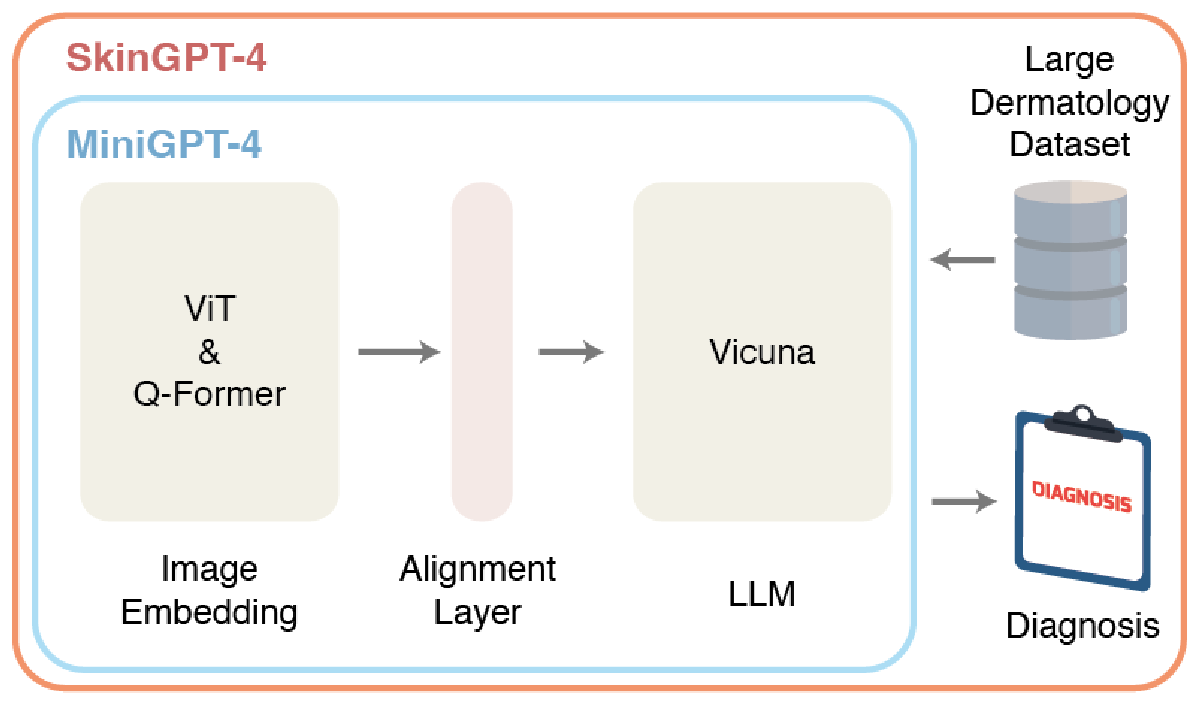
\includegraphics[width=0.55\columnwidth,keepaspectratio]{images/skingpt4.png}
    \caption{\small Arquitetura do Skin\ac{GPT}-4. Fonte: \textcite{zhou2023skingpt}.}
    \label{fig:skingpt4}
\end{figure}

Nesse estudo, o Mini\ac{GPT}-4 passou por um processo de \textit{fine-tuning} de duas etapas que familiarizou o modelo com imagens de lesões de pele e depois ajustou suas
saídas para um formato mais próximo de um diagnóstico médico. As imagens vieram de um conjunto de dados particular, do SKINCON e do Dermnet, sendo que 3886 imagens foram
usadas na primeira etapa de treinamento e 49043 na segunda.

A verificação do desempenho do modelo foi feito com base em 150 diagnósticos de casos reais realizados pelo Skin\ac{GPT}-4. Esses diagnósticos foram avaliados por
dermatologistas certificados, sendo que 78,76\% dos diagnósticos foram classificados como corretos.

\subsection{LLaVA-Med}

O \ac{LLaVA}-Med é um modelo com foco na área médica geral desenvolvido por \textcite{li2024llava}. Esse modelo é baseado no \ac{LLaVA}, sendo composto pelo \ac{LLM}
Vicuna e o codificador visual \ac{CLIP} \ac{ViT}-L/14 \cite{liu2024visual}.

Foram criados dois conjuntos de dados com base em pares de imagens e textos de diversas áreas da medicina, um conjunto para alinhamento de conceitos e outro para
\textit{instruction-following}. A primeira etapa do treinamento envolveu o \textit{fine-tuning} do projetor de entrada por 7 horas em 8 NVIDIA A100 de 40 GB, alinhando
o modelo com o contexto médico. Já a segunda etapa levou 8 horas com as mesmas GPUs, realizando o \textit{fine-tuning} sobre o projetor de entrada e o \ac{LLM}, adaptando
o modelo para responder perguntas sobre imagens de casos médicos.

Esse modelo apresentou um desempenho melhor em relação ao \ac{LLaVA} original, atingindo mais de 90 pontos no \textit{benchmark} PathVQA, por exemplo.

\subsection{MpoxVLM}

O modelo MpoxVLM de \textcite{cao2024mpoxvlm} é um \ac{MLLM} direcionado ao diagnóstico de lesões de pele causadas pela doença \textit{Monkeypox}. O modelo possui dois
codificadores visuais, um deles é o \ac{CLIP} \ac{ViT}-L/14 e o outro é o \ac{ViT}-L/14-336 pré-treinado para a classificação de lesões de pele. Um \ac{MLP} de duas camadas
é usado como projetor de entrada para o codificador \ac{CLIP}, sendo que a saída do codificador \ac{ViT}, a classe da lesão de pele, é enviada para outro projetor de
entrada. O \ac{LLaMA}-2 é usado como \ac{LLM}, especificamente a variante com 7 bilhões de parâmetros. A \autoref{fig:mpoxvlm} apresenta a arquitetura deste \ac{MLLM}.

\begin{figure}[ht]
    \centering
    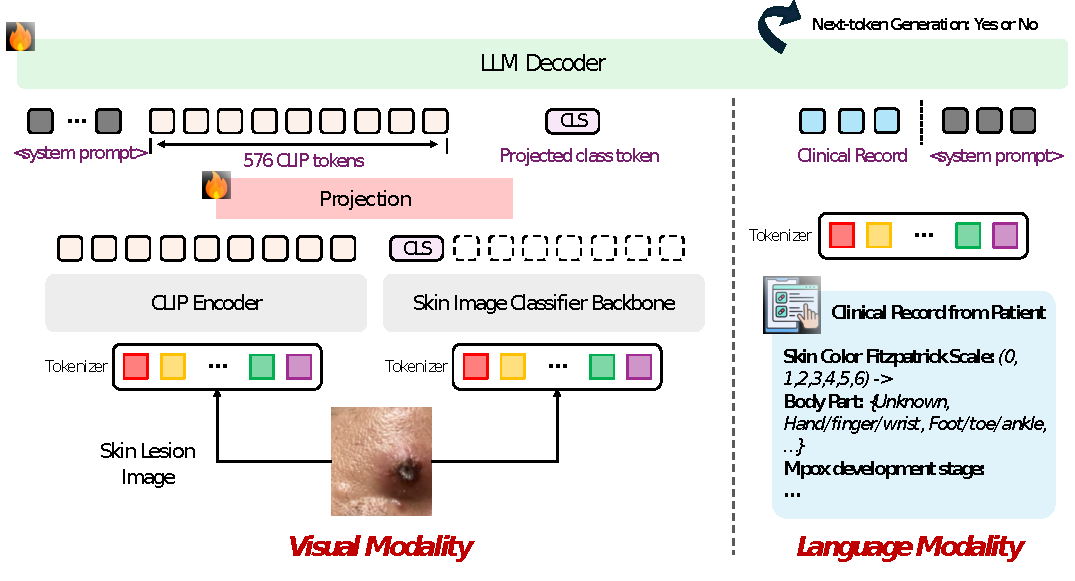
\includegraphics[width=0.85\columnwidth,keepaspectratio]{images/mpoxvlm.pdf}
    \caption{\small Arquitetura do MpoxVLM. Fonte: \textcite{cao2024mpoxvlm}.}
    \label{fig:mpoxvlm}
\end{figure}

Inicialmente, o \ac{ViT}-L/14-336 foi pré-treinado com o conjunto de dados de lesões de pele causadas por \textit{Monkeypox}. Depois o modelo foi construído e os
projetores de entrada foram treinados. Por fim, foi feito um \textit{fine-tuning} com \ac{LoRA} do \ac{LLaMA}-2 para tarefas de pergunta e resposta. Foram utilizadas
duas NVIDIA RTX 4090 para os treinamentos nesse estudo.

Os resultados apresentados demonstram que o MpoxVLM atinge uma acurácia de 90,38\% no diagnóstico de \textit{Monkeypox}, ultrapassando vários outros \acp{MLLM}.

\subsection{Comparação entre MLLMs} % TODO: Comentar que no paper do LLaMA-3.2 viram que CLIP não é tão bom assim

Em geral, os modelos utilizam como base \acp{LLM} da família \ac{LLaMA} e codificadores visuais baseados em \acp{ViT}, sendo que o MpoxVLM apresentou a arquitetura
mais complexa. O \textit{fine-tuning} completo também é frequentemente utilizado, porém, o MpoxVLM atingiu bons resultados com o \ac{LoRA}. Dos três modelos apresentados,
somente o Skin\ac{GPT}-4 e o MpoxVLM são especializados em lesões de pele, sendo que o artigo do Skin\ac{GPT}-4 é o que tem o objetivo mais similar ao deste trabalho. Os
conjuntos de dados utilizados são diversos e possuem imagens de diferentes categorias, como macroscópicas e dermatoscópicas.

Devido a recência do \ac{LLaMA}-3.2, há poucos casos em que este modelo foi utilizado. Um diferencial considerável deste trabalho é a utilização deste \ac{MLLM}. Outro
diferencial é a análise da eficácia do \ac{QLoRA} em relação ao \ac{LoRA} no contexto de classificação de lesões de pele. A \autoref{tab:mllm_comparison} mostra uma
comparação entre os \acp{MLLM} apresentados.

\begin{table}[ht]
    \caption{\small Comparação entre diferentes \acp{MLLM} focados na área médica e na classificação de lesões de pele.}
    \centering
    \begin{tabular}{l|cc}
        \hline
        Modelo                & MLLM base ou arquitetura                  & Treinamento            \\ \hline
        Skin\ac{GPT}-4        & Mini\ac{GPT}-4                            & Fine-tuning completo   \\
        \ac{LLaVA}-Med        & \ac{LLaVA}                                & Fine-tuning completo   \\
        MpoxVLM               & \ac{CLIP}, \ac{ViT}-L/14-336 e LLaMA-2-7B & \ac{LoRA}              \\
        Modelo deste trabalho & \ac{LLaMA}-3.2-11B e \ac{LLaMA}-3.2-90B   & \ac{QLoRA} e \ac{LoRA} \\ \hline
    \end{tabular}
    \label{tab:mllm_comparison}
    \fonte{Autoria própria.}
\end{table}